\documentclass[a4paper]{article}

%% Language and font encodings
\usepackage[english]{babel}
\usepackage[utf8x]{inputenc}
\usepackage[T1]{fontenc}

%% Sets page size and margins
\usepackage[a4paper,top=3cm,bottom=2cm,left=3cm,right=3cm,marginparwidth=1.75cm]{geometry}

%% Useful packages
\usepackage{amsmath}
\usepackage{graphicx}
\usepackage[colorinlistoftodos]{todonotes}
\usepackage[colorlinks=true, allcolors=blue]{hyperref}
\usepackage{float}
\usepackage{listings}
\usepackage{algorithm2e}
\usepackage{mathtools}
\DeclarePairedDelimiter\ceil{\lceil}{\rceil}
\DeclarePairedDelimiter\floor{\lfloor}{\rfloor}

%opening
\title{Assignment 1}
\author{Shruti Shivakumar}

\begin{document}
\maketitle

\section{Algorithm Design and Complexity}
\subsection{}
If $k \geq \ceil*{\log (n)}$, then the algorithm would be a binary search of the floors of the building. If the box does not break from the $n$ floor, then the index is $n+1$. Else, set lowest possible floor as 1 and the highest possible floor as $n$. If the box breaks in a floor $mid$ halfway between the lowest possible and highest possible, then reset the highest possible floor as $mid$. Else if the box does not break at $mid$, then reset the lowest possible floor as $mid$. Repeat the procedure till the lowest possible and highest possible floors are adjacent to each other, then the index is the highest possible floor. This algorithm will have a cost complexity of $\mathcal{O}(\log n)$
\subsection{}
If $k \leq \ceil*{\log (n)}$, then the algorithm would be a binary search of the floors until we exhaust $k-1$ boxes followed by a simple linear search from the lowest untested floor till we reach the highest untested floor. The floor where the box breaks is the required index. The first part of the algorithm will have a cost complexity of $\mathcal{O}(\frac{n}{2^{k-1}})$. The second part has a cost complexity of $\mathcal{O}(k)$. Thus, the algorithm has a complexity of $\mathcal{O}(\frac{n}{2^{k-1}} + k)$. 
\subsection{}
For $k=2$, divide the $n$ floors into subsets of $\sqrt{n}$ consecutive floors. Start from the highest floor of the lowest unchecked subset and test if the box breaks. If it does, then test for box breakage from each floor starting from the lowest floor in that subset. The floor where the box breaks is the index. If the box does not break in the highest floor of the given subset, move on to the next lowest unchecked subset and repeat procedure. This algorithm will have a cost complexity of $\mathcal{O}(\sqrt{n})$
\section{Greedy 1}
\subsection*{Algorithm}
Greedy algorithm to minimise the number of sealant strips of length $L$ such that all $n$ holes along the pipe are covered :
\begin{itemize}
\item Fix the leftmost end of the pipe as $START$
\item Sort the holes in the order of increasing distance from $START$
\item Looping through the sorted holes list :
\begin{itemize}
\item If the hole is not covered yet, plaster the sealant strip starting from that hole position $START-HOLE$ and covering all points within distance $L$ to the right of the hole. Increment number of sealants
\end{itemize}
\end{itemize}
\subsection*{Time Complexity}
The time complexity of the algorithm $T = T_{1} + T_{2}$, where $T_{1} = $ Time complexity of sorting the list $ = \mathcal{O}(n \log n)$ and $T_{2} = $ Time complexity of checking if hole lies within distance $L$ of the hole from which sealant strip starts$ = \mathcal{O}(n)$. Thus, $T = \mathcal{O}(n \log n)$.
\subsection*{Proving correctness}
Note that the problem instance here is to choose $START-HOLE$ from the given set of uncovered holes such that the number of sealant strips used is minimsed. Thus we need to show that for every problem instance $X$, there exists an optimal greedy solution that includes the first greedy choice $x$ picked by the algorithm. Let $Q$ be any optimal solution to $X$. $x$ is the uncovered hole closest to $START$ chosen from the given set of uncovered holes in the problem instance. If $x$ belongs to $Q$, then proved. Else $Q$ instead adds $y$ to the optimal solution. Now, $y$ cannot be within $L$ distance to the right of $x$ else the sealant strip used to cover $x$ will overlap with that used to cover $y$. So, instead of covering $x$ and $y$ with one sealant strip, we are using two which is not optimal. Thus, $y$ lies at a distance greater than $L$ to the right of $x$. Construct a solution $Q^{'}$ that subtitutes $y$ with $x$. Since both $Q$ and $Q^{'}$ add one sealant to the solution, if $Q$ is optimal, $Q^{'}$ is also optimal. \\
To prove optimal substructure property, we need to show that if $Y$ is the subproblem left from $X$ after greedy choice $x$ and if $R$ is the optimal solution to $Y$, then $Q = R \cup {x}$ is an optimal solution to $X$. Now, the $N_{sealants}(Q) = N_{sealants}(R) + 1$. If $Q$ is not optimal, then let $Q^{'}$ be an optimal greedy solution to $X$ that uses the initial greedy choice $x$. Now, once $x$ along with all the holes within $L$ distance to the right of $x$ is removed from the set of uncovered holes, the new problem instance, $Y$, has a solution that uses lower number of sealants than $R$. This is not possible. Thus, $Q$ is an optimal solution to $X$.

\section{Greedy 2}
\subsection*{Algorithm}
Greedy algorithm to maximise the value of the bag while ensuring that its weight does not exceed $L$ :
\begin{itemize}
\item Sort the minerals in descending order according to the ratio of their value to weight
\item Initialise current weight of bag = 0
\item Looping through the sorted minerals list :
\begin{itemize}
\item If adding the entire mineral will not result in the bag's weight exceeding $L$, add entire mineral to bag
\item Else add the fraction of the mineral which will completely fill the bag
\end{itemize}
\end{itemize}
\subsection*{Proving optimality}
Note that the problem instance here is to choose minerals from the given set that will maximise the bag's value while ensuring that its weight does not exceed $L$. Thus we need to show that for every problem instance $X$, there exists an optimal greedy solution that includes the first greedy choice $x$ picked by the algorithm. Let $Q$ be any optimal solution to $X$. $x$ is maximum weight that can be added to the bag of the mineral $m$ with the highest value to weight ratio for that problem instance. If $x$ belongs to $Q$, then proved. Else $Q$ instead adds weight $w<x$ of $m$. Now, $Q$ must have atleast $r = x-w$ weight of minerals other than $m$ in the bag. Let $Q^{'}$ be the solution obtained by substituting $r$ weight of other minerals with $r$ weight of mineral $m$. Since $m$ has highest value to weight ratio, the $Q^{'}$ has a value atleast as large as $Q$. Thus, $Q^{'}$, which is the greedy solution, is also optimal.


\section{Minimum Spanning Tree Implementation}
\subsection*{Static Computation - computeMST()}
I implemented Prim's algorithm to find MST of the given graph. For the minimum priority queue data structure used in the algorithm, I decided to use a Fibonacci heap \cite{fibo} instead of a binary min-heap. With a binary min-heap, Prim's algorithm gives a time complexity of $\mathcal{O}(V\log V + E\log E)$ since it takes $\mathcal{O}(\log V)$ to get the vertex with the least key in the queue and $\mathcal{O}(\log E)$ to decrease the key of an edge in the queue. However, a Fibonacci heap, the decrease key operation of an edge takes $\mathcal{O}(1)$ time, resulting in overall time complexity of $\mathcal{O}(V\log V + E)$.
\subsection*{Dynamic Computation - recomputeMST()}
The algorithm behind $recomputeMST()$ is as follows. Given a new edge $e$ of weight $w$ to be added between vertices $u$ and $v$, the algorithm first computes the path from $u$ to $v$ along the MST. If the maximum-weighted edge $e'$ along this path has a weight greater than $w$, then $e'$ is removed from the MST and $e$ is added. If one of $u$ (or $v$) is a new vertex, then the edge $e$ is simply added to the MST (and thus the graph). Note that both $u$ and $v$ cannot be new vertices, else the no MST would be possible in the new graph. The time complexity of the algorithm is the time taken to compute the path from $u$ to $v$ i.e the time taken for a breadth first search from $u$ to $v$ along the MST, which is $\mathcal{O}(E_{MST} + V) = \mathcal{O}(V-1 + V) = \mathcal{O}(V)$
\subsection*{Plotting running time}
\begin{figure}[H]
\centering
    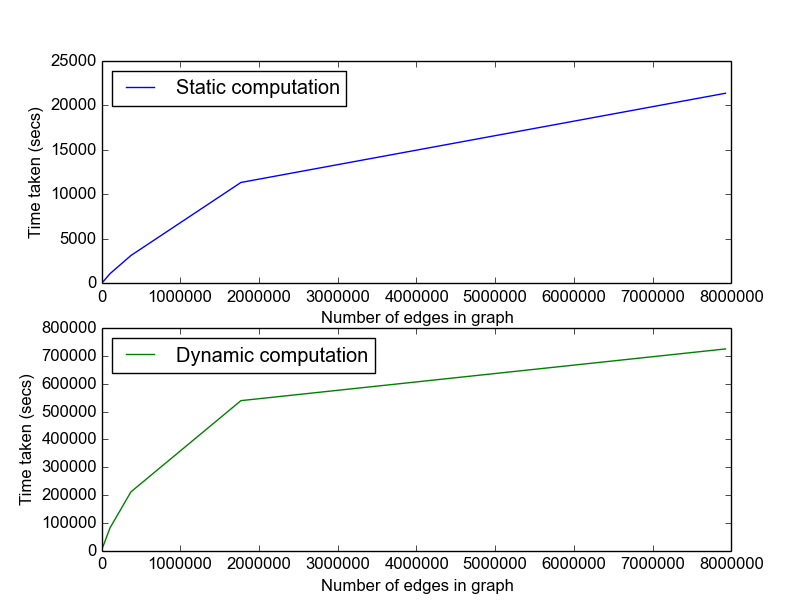
\includegraphics[width=0.75\textwidth]{../results/Plot.png}
    \caption{Plot of running time of static and dynamic computation of MST with increasing number of edges in graph}
    \label{fig:plot}
\end{figure}
The plots of both static and dynamic computation increase with number of edges in the graph. Since the number of vertices is also increasing per graph, the empirical scaling observed does match the $\mathcal{O}$-analysis. However, since we are evaluating the dynamic computation function everytime we add an edge, dynamic computation is more expensive than static even though its theoretical complexity is better than the complexity of static computation.

\begin{thebibliography}{9}
\bibitem{fibo} 
Keith Schwarz.
\textit{fibonacci-heap-mod 1.0 : A Pure Python Fibonacci Heap implementation of a Priority Queue}. 
Ported to Python by Daniel Stromberg
\\\texttt{https://pypi.python.org/pypi/fibonacci-heap-mod/}, 2017.

\end{thebibliography}
\end{document}
